%%%%%%%%%%%%%%%%%%%%%%%%%%%%%%%%%%%%%%%%%%%%%%%%%%%%%%%%%%%%%%%%%%%%%%%%%%%%%%%%
% \documentclass[12pt,papel,twoside]{ibtesis}
\documentclass[12pt,screen,twoside]{ibtesis}
% \documentclass[12pt,papel,singlespace,oneside]{ibtesis}
% \documentclass[12pt,papel,preprint,singlespace,oneside]{ibtesis}


%%%%%%%%%%%%%%%%%%%%% Paquetes extra %%%%%%%%%%%%%%%%%%%%%%%%%%%%%%%%%%%%%%%%%%%
% Por conveniencia: aqu\'{\i} puede cargar todos los paquetes y definir los comandos 
% que necesite
%\usepackage{ibextra}

\usepackage[utf8]{inputenc}
\usepackage[dvipsnames]{xcolor} %Si quisieramos poner texto en color
\usepackage{float} %para poner Here en imagen
\usepackage{graphicx} %para insertar imágenes
\usepackage{subfig}
%\usepackage{ibextra}
                % Archivo de bibliografía


%%%%%%%%%%%%%%%%%%%%%%%%%%%%%%%%%%%%%%%%%%%%%%%%%%%%%%%%%%%%%%%%%%%%%%%%%%%%%%%%
%%%%%%%%%%%%%%%%%%%%% Informacion sobre la tesis %%%%%%%%%%%%%%%%%%%%%%%%%%%%%%%
\title{Análisis del Flujo en Convección Mixta en Canales Rectangulares}
\author{Patricio G. Canciani}
\director{Dr. William I. Machaca Abregu}
\codirector{Dr. Federico Teruel}
\carrera{Tesis Carrera de Maestría en Ingeniería}
\grado{Maestrando}
\laboratorio{Departamento de Mecánica Computacional \\ (Centro Atómico Bariloche)}
\jurado{Dr. Christian P. Marcel (Instituto Balseiro -- CNEA)\\ 
Dr. Pablo Garcia Martinez (Instituto Balseiro -- CNEA)\\ 
Dr. César Venier (FCEIA -- SIMEC)\\}

\palabrasclave{Flujo Turbulento,Convección Mixta}
\keywords{Turbulent Flow, Mixed Convection}
% Si queremos poner la fecha manualmente:
% \date{Diciembre de 2099}

%%%%%%%%%%%%%%%%%%%%%%%%%%%%%%%%%%%%%%%%%%%%%%%%%%%%%%%%%%%%%%%%%%%%%%%%%%%%%%%%
%\titlepagefalse % Si no quiere compilar la portada descomente esta linea
%\includeonly{apendices} % Compilar s\'{o}lo estos archivos 
\graphicspath{{figs/}} % Lugar donde encontrar las figuras generales (se puede poner uno en cada cap{\'{\i}}tulo)
%%%%%%%%%%%%%%%%%%%%%%%%%%%%%%%%%%%%%%%%%%%%%%%%%%%%%%%%%%%%%%%%%%%%%%%%%%%%%%%%


\begin{document}

% Dentro del environment 'preliminary' va:
% la dedicatoria, resumen, abstract, indices

\begin{preliminary}

% Escriba su dedicatoria
\dedicatoria{
A mi padres\\
A mi hermana\\
A mis amigos\\
A todos mis seres queridos}

%%% \'{I}ndices %%%%

\begin{abreviaturas}
                                %Abreviaturas
\end{abreviaturas}

\tableofcontents                %\'{I}ndice

\listoffigures                  %Figuras

\listoftables                   %Tablas

\begin{resumen}%

La convección mixta en conductos verticales está presente en numerosos sistemas de interés, entre ellos los intercambiadores de calor. Estos sistemas pueden presentar cambios de régimen (laminar-turbulento) durante su funcionamiento. Esto es relevante ya que el coeficiente de fricción ($f$) o el número de Nusselt (Nu) pueden experimentar grandes variaciones. En el presente trabajo se estudia la evolución temporal de magnitudes de interés durante la transición desde el régimen laminar hacia el turbulento, para un canal vertical de placas paralelas con flujo de calor constante en las paredes.

Para estudiar la transición temporal, primero resulta necesario conocer el estado inicial laminar y el estado final turbulento. En ese sentido, se analiza el flujo turbulento completamente desarrollado bajo la influencia de la fuerza boyante. Tanto el estudio del estado turbulento desarrollado como la transición temporal laminar-turbulenta se realiza mediante simulaciones DNS empleando Xcompact3D. 

Las condiciones iniciales que inducen la inestabilidad se obtienen mediante análisis de estabilidad lineal, resolviendo el problema de autovalores y autofunciones derivado de las ecuaciones de Orr-Sommerfeld para convección mixta. Esta resolución se realiza con la herramienta OSMC desarrollada en el grupo MECOM. Las soluciones permiten desencadenar la transición para examinar su evolución temporal. 


En el análisis del régimen turbulento desarrollado se consideran $2100 \leq \mathrm{Re}_o \leq 5000$ \textcolor{black}{(número de Reynolds basado en el semiancho del canal y la velocidad en el centro)}, \linebreak $\mathrm{Pr}=0\text{.}071,0\text{.}71$ \textcolor{black}{(número de Prandtl)} y $0\text{.}04 \leq \mathrm{Ri}_b \leq 106\text{.}5$  \textcolor{black}{(número de \linebreak Richardson  basado en el ancho del canal y la velocidad \textit{bulk})}. Para $\mathrm{Re}_o=5000$ y $\mathrm{Pr}=0\text{.}71$ se  analizan perfiles de cantidades medias y fluctuaciones. Las estimaciones de Nu  concuerdan con correlaciones de la literatura en los rangos estudiados. \textcolor{black}{Se identifica una región del número de boyancia ($10^{-6} \lesssim \text{Bo} \lesssim 3 \times 10^{-5}$), el cual cuantifica la relación entre las fuerzas boyantes y la fuerza impulsora de la convección forzada,} donde Nu disminuye respecto de la convección puramente forzada, asociado a una menor producción de turbulencia próxima a las paredes. Se propone asimismo una correlación empírica para el factor de Darcy ($f$) con buen acuerdo frente a datos y referencias.

La transición laminar-turbulenta se examina para $\mathrm{Re}_o=5000$, $\mathrm{Pr}=0\text{.}71$ y dos intensidades de boyancia ($\mathrm{Ri}_b=0\text{.}04$ y $\mathrm{Ri}_b=1\text{.}06$). Se identifican combinaciones de perturbaciones que inducen la transición y se observa que una mayor boyancia incrementa la inestabilidad del flujo. Las cantidades TKE \textcolor{black}{(Energía Cinética Turbulenta)}, varianza de temperatura, Nu y $f$ muestran respuestas transitorias no monótonas; en el caso de mayor $\mathrm{Ri}_b$ se registra una caída pronunciada de Nu concurrente con aumento de TKE y el aplanamiento del perfil de velocidad por efecto de la turbulencia. Finalmente, se observa que el valor del estado turbulento desarrollado de $\mathrm{Re}_\tau$ \textcolor{black}{(número de Reyndols de fricción)} se encuentra por encima del valor asociado al estado inicial en el caso de $\mathrm{Ri}_b$ menor y por debajo en el de $\mathrm{Ri}_b$ mayor.

\end{resumen}


\begin{abstract}%

Mixed convection in vertical ducts is present in numerous systems of interest, including heat exchangers. These systems may undergo regime changes (laminar–turbulent) during operation. This is relevant since the friction coefficient ($f$) or the Nusselt number (Nu) may exhibit large variations. In the present work, the temporal evolution of quantities of interest is studied during the transition from the laminar regime to the turbulent one, for a vertical parallel-plate channel with constant wall heat flux.

To investigate the temporal transition, it is first necessary to characterize both the initial laminar state and the final turbulent state. In this regard, the fully developed turbulent flow under the influence of buoyancy is analyzed. Both the study of the developed turbulent state and the laminar–turbulent temporal transition are carried out through DNS simulations using Xcompact3D. 

The initial conditions that trigger the instability are obtained by means of linear stability analysis, solving the eigenvalue and eigenfunction problem derived from the Orr–Sommerfeld equations for mixed convection. This resolution is performed with the OSMC tool developed in the MECOM group. The solutions allow the transition to be triggered in order to examine its temporal evolution. 



In the analysis of the developed turbulent regime, $2100 \leq \mathrm{Re}_o \leq 5000$ \textcolor{black}{(Reynolds number based on the channel half-width and the centerline velocity)}, \linebreak $\mathrm{Pr}=0\text{.}071,0\text{.}71$ \textcolor{black}{(Prandtl number)} and $0\text{.}04 \leq \mathrm{Ri}_b \leq 106\text{.}5$ \textcolor{black}{(Richardson number based on the channel width and the bulk velocity)} are considered. For $\mathrm{Re}_o=5000$ and $\mathrm{Pr}=0\text{.}71$, mean and fluctuating quantities are analyzed. The estimates of Nu agree with correlations from the literature within the studied ranges. \textcolor{black}{A region of the buoyancy number ($10^{-6} \lesssim \text{Bo} \lesssim 3 \times 10^{-5}$), which quantifies the relationship between buoyancy forces and the driving force of forced convection,} is identified where Nu decreases with respect to purely forced convection, associated with a lower turbulence production near the walls. An empirical correlation for the Darcy friction factor ($f$) is also proposed, showing good agreement with data and references.

The laminar–turbulent transition is examined for $\mathrm{Re}_o=5000$, $\mathrm{Pr}=0\text{.}71$, and two buoyancy intensities ($\mathrm{Ri}_b=0\text{.}04$ and $\mathrm{Ri}_b=1\text{.}06$). Combinations of perturbations that induce transition are identified, and it is observed that higher buoyancy increases the flow instability. The TKE \textcolor{black}{(Turbulent Kinetic Energy)}, temperature variance, Nu, and $f$ exhibit non-monotonic transient responses; in the case with higher $\mathrm{Ri}b$, a sharp decrease in Nu is recorded, concurrent with an increase in TKE and a flattening of the velocity profile due to turbulence. Finally, it is observed that the value of the developed turbulent-state $\mathrm{Re}\tau$ \textcolor{black}{(friction Reynolds number)} lies above the value associated with the initial state for the lower $\mathrm{Ri}_b$ case and below for the higher $\mathrm{Ri}_b$ case.


\end{abstract}



%%% Local Variables: 
%%% mode: latex
%%% TeX-master: "template"
%%% End: 


\end{preliminary}


% Podemos usar cualquiera de los dos comandos: \input o \include para incluir el texto
\chapter{Introducción}
\label{intro}
%\chapterquote{Hablaban siempre de dinero y planeaban asaltar un banco}{Domingo Cavallo, 2001}

Capitulo introductorio de la tesis


Algunas preguntas clave que deberian responderse en este capitulo:

¿Cuál es el campo general de estudio de tu tesis?

¿Qué fenómeno, problema o sistema estás investigando?

¿Por qué este tema es relevante científica o tecnológicamente?

¿Qué problema específico intenta resolver tu tesis?

¿Cuáles son los objetivos (generales y/o específicos)?

¿Qué enfoque metodológico utilizás? ¿Experimental, teórico, computacional?

¿Cómo está organizada la tesis?

\newpage
\section{Introducción}

Un fluido, en virtud de su masa y velocidad, puede transportar momento. Además, en virtud de su temperatura, puede transportar calor. Estrictamente hablando, la convección es el transporte de energía debido al movimiento global de un medio. Sin embargo, en ingeniería es común utilizar el término convección de forma más amplia para describir la transferencia de calor desde una superficie hacia un fluido en movimiento cuando ambos están a diferentes temperaturas \cite{cengelheat,incropera}. 

La transferencia de calor por convección puede clasificarse según la naturaleza del flujo. Hablamos de convección forzada cuando el flujo es provocado por actores externos como puede ser la acción de bombeo o un gradiente de presión; en cambio, en la convección natural, el flujo es inducido por fuerzas boyantes o de flotación, las cuales se deben a diferencias de densidad producidas por variaciones de temperatura en el propio fluido (Figura \ref{fig:natural_forzada}).

\begin{figure}[H]
 \centering
    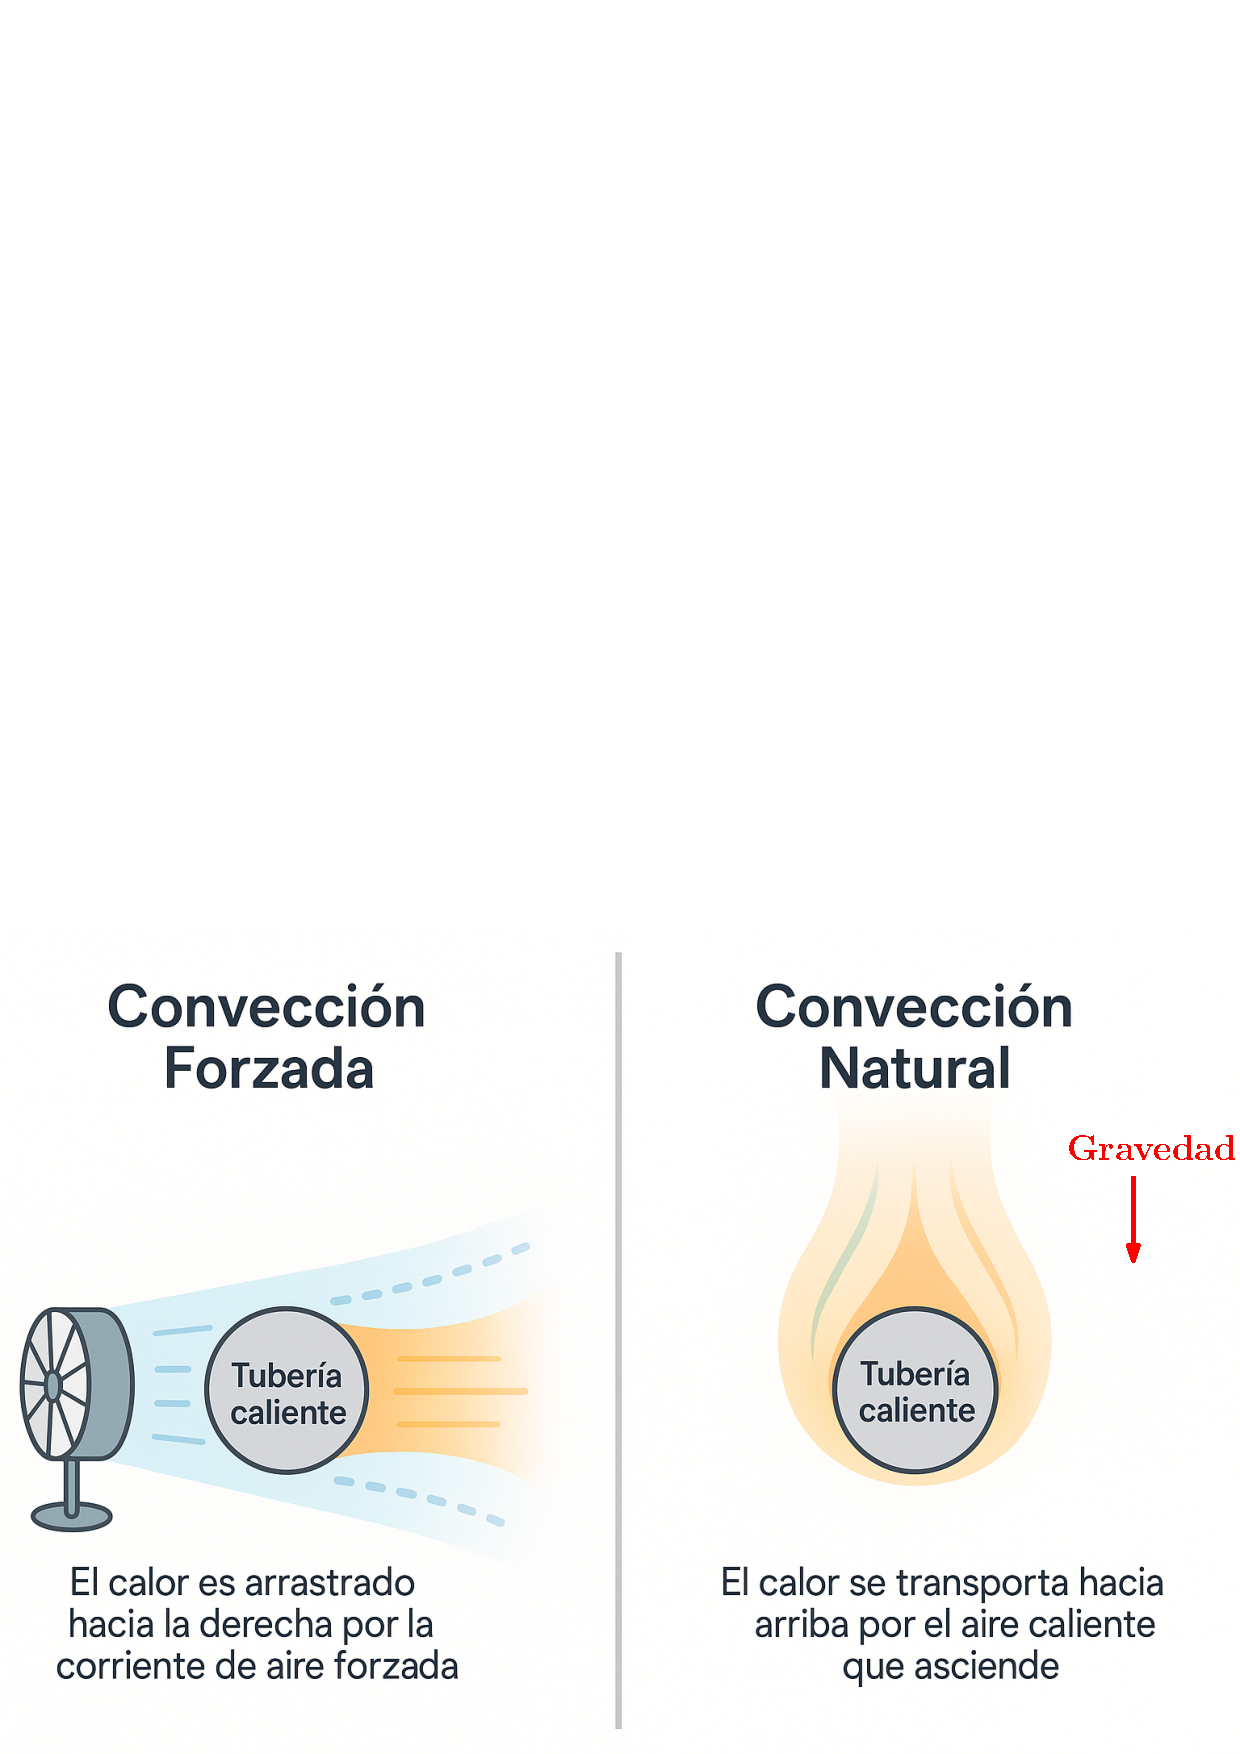
\includegraphics[width=0.6\textwidth]{figures/cap1/natural_forzada.png}
    \label{fig:natural_forzada} 
 \caption{Comparación esquemática de la transferencia de calor alrededor de una tubería caliente: (izquierda) convección forzada; (derecha) convección natural.} 
 \label{fig:natural_forzada}
\end{figure}


Los primeros estudios sobre la transferencia de calor por convección trataron las ramas de la convección forzada y la convección natural de forma separada, sin considerar la posible interacción entre ambas. Por un lado, los experimentos de Henri Bénard (1901) marcaron un hito en la comprensión de la convección natural \cite{benard1901}. Más tarde, Lord Rayleigh (1916) desarrolló la base teórica de la inestabilidad térmica en capas fluidas \cite{rayleigh1916}. En paralelo, en el ámbito de la convección forzada, trabajos como el de Dittus y Boelter (1930) establecieron correlaciones empíricas para la transferencia de calor en tubos \cite{dittus1930}. No fue sino hasta mediados del siglo XX que comenzó a reconocerse que ambos mecanismos pueden coexistir en muchas configuraciones de interés práctico. Así surgió el concepto de convección mixta, donde la convección forzada y la natural actúan simultáneamente como casos extremos de un fenómeno más general \cite{tao1960,metais1964}. 

Por otra parte, cuando un fluido se desplaza a través de un conducto o sobre una superficie, su movimiento puede clasificarse en dos tipos de régimen: laminar o turbulento. En el régimen laminar, el flujo es ordenado y las partículas del fluido se mueven en capas paralelas sin mezclarse entre sí. En cambio, en el régimen turbulento, el flujo es caótico, con remolinos, mezclas intensas y fluctuaciones en velocidad y presión. Un flujo se encuentra en un estado de transición desarrollado (esto es, no varía con el tiempo o con el espacio en un sentido de promedio estadístico), se dice que el flujo está en régimen de transición. Por otro lado, la evolución del flujo laminar a un flujo turbulento completamente desarrollado es llamada transición laminar-turbulenta. Esta transición puede ocurrir en el tiempo (transición laminar-turbulenta temporal) o en el espacio (transición laminar-turbulenta espacial).

La transición laminar-turbulenta es un fenómeno de gran importancia para la ingeniería y la física aplicada ya que puede ocurrir en diferentes dispositivos termohidráulicos. El cambio de un régimen a otro puede tener un impacto significativo en la transferencia de calor, especialmente en aplicaciones de convección mixta. El coeficiente de fricción (factor de Darcy) o el coeficiente de convección (numéro de Nusselt) se incrementan notablemente cuando se produce la transición \cite{incropera,white}. Por ejemplo, un problema importante se da en el diseño de intercambiadores de calor cuando el punto de trabajo del flujo dentro de los tubos se encuentra en régimen de transición, que es, en general, un estado intermitente en el cual parámetros tales como el coeficiente de fricción y el coeficiente de transferencia de calor tienen una gran variación \cite{ghajar2019heat}.



\textcolor{red}{Hay que poner un poco de revision bilbiografica de analisis de estabilidad lineal, capaz ... y también de revisión numerico}




\section{Motivación}


En la actualidad, muchos problemas de ingeniería presentan flujos en régimen de transición. Por citar algunos ejemplos tenemos los álabes de una turbina o los intercambiadores de calor. La mayoría de los flujos en estás condiciones son no isotérmicos \cite{chen2003direct}. 

Desde el punto de vista ingenieril, si bien éste es un régimen de trabajo no deseado por ser un estado intermitente, las características del mismo son de gran relevancia


El estudio de la transferencia de calor en la transición laminar-turbulenta es importante en diversas aplicaciones ingenieriles, como en los elementos combustibles de reactores nucleares de investigación, en intercambiadores de calor y en equipos electrónicos, entre otros. Si bien el régimen de transición no es deseado desde el punto de vista ingenieril ya que es intermitente (es decir, el flujo puede fluctuar
entre los regímenes laminar y turbulento), el estudio de la transición es relevante para poder controlar el fenómeno o anticipar, y por tanto aprovechar, su comportamiento.


La convección forzada y la convección natural son dos modos distintos de convección, que suelen combinarse y manifestarse conjuntamente en flujos ambientales y aplicaciones de ingeniería. El fenómeno de convección mixta  ocurre en procesos de fabricación de silicio, refrigeración de equipos electrónicos, paneles solares térmicos, álabes de turbinas, intercambiadores de calor de diverso tipo, reactores nucleares, entre otros \cite{kasagi1997direct}. 

Entre las aplicaciones técnicas de mayor relevancia de la convección mixta se destaca el transporte de energía térmica. En este sentido, las necesidades energéticas actuales propician el diseño y mejora constante de los reactores nucleares utilizados para la provisión de energía eléctrica. Dentro de la nueva generación de reactores nucleares GEN-IV (\url{https://www.gen-4.org/}), de los seis conceptos
especificados, uno corresponde a reactores tipo GFR (\textit{Gas-cooled Fast Reactor}) que utiliza como refrigerante gas helio cuyo numero de Prandtl es Pr$\simeq0.7$ similar al aire.





En las últimas décadas se han realizado muchos esfuerzos para desarrollar técnicas
tendientes a mejorar la transferencia de calor y el desempeño global de los intercambia-
dores de calor. El interés en estas técnicas radica en el ahorro de la energía. Con este
objetivo, se realizaron experimentos tanto en tubos como en canales, para determinar
experimentalmente las correlaciones de transferencia de calor.


Por otro lado, el estudio de la transferencia de calor en canales rectangulares ha
ganado interés en los últimos años, motivado por su aplicación en combustibles de
núcleos de reactores de investigación, en el área de sistemas electrónicos avanzados por el sistema de refrigeración



\section{Objetivos}

\section{Organización del trabajo}
\chapter{Modelado Computacional y XC3D}

\section{Metodos Numéricos}

\section{Xcompact3D}
\cite{kawamura2000dns}
\section{Modelo Computacional}

\cite{moser1999}




\chapter{Herramientas Numéricas} \label{cap:numerico}

En este capítulo se da una breve descripción de las herramientas numéricas utilizadas: Xcompact3D y OSMC. Xcompact3D resuelve las ecuaciones de Navier-Stokes junto a la ecuación de transporte de un escalar, brindando la capacidad de resolver en forma eficiente y precisa flujos turbulentos en canales rectangulares usando una grilla cartesiana simple; además, es una herramienta popular en el ámbito de la investigación básica y aplicada. Una descripción completa de la misma puede encontrarse en \url{https://www.incompact3d.com/}.

Por su parte, OSMC se emplea para resolver el problema de autovalores y autofunciones detallado en la sección \ref{sec:estabilidad}. El mismo utiliza el método espectral de Colocación de la Matriz de Chebyshev transformando el problema original a un problema autovalores y autovectores. Esta herramienta fue desarrollada por Pablo Szuban \cite{szuban2023} en el grupo de Mecánica Computacional (MECOM-CAB). 


\section{Xcompact3D (XC3D)}

Comprender, predecir y controlar los flujos turbulentos es crucial, y a la vez, un factor relevante en la industria, no en vano sigue siendo uno de los desafíos más complejos en investigación. Además, el diseño de numerosos sistemas de ingeniería e industriales, así como la evaluación de su impacto ambiental, depende de cuantificar con precisión el comportamiento turbulento de los flujos.

Si bien las ecuaciones de Navier-Stokes constituyen el modelo matemático de referencia para describir la dinámica de un flujo turbulento, su resolución es especialmente exigente debido al carácter caótico y multiescala de la turbulencia \cite{pope2001turbulent}. Las escalas relevantes abarcan varios órdenes de magnitud y demandan elevados recursos de cómputo y memoria. El notable incremento en las últimas dos décadas en la capacidad computacional ha impulsado el uso de simulaciones de alta fidelidad; en particular, las simulaciones DNS\footnote{Simulaciones numéricas en las que se resuelve la gran mayoría de las escalas turbulentas.} se han consolidado como una herramienta clave para la predicción de flujos y se ha convertido, junto al CFD\footnote{\textit{Computational Fluid Dynamics}}, en un complemento esencial de la teoría y el experimento.

En este trabajo se estudian el flujo de un fluido, y la transferencia de calor en régimen turbulento con convección mixta, así como la transición laminar-turbulenta temporal, mediante simulaciones numéricas directas. Ello exige resolver las ecuaciones de Navier-Stokes y de transporte de un escalar, acopladas entre sí, con alta precisión numérica y eficiencia computacional. Para este fin se emplea Xcompact3D\footnote{Abreviado en este trabajo como XC3D}, una herramienta numérica implementada en Fortran 90/95 orientada a arquitecturas basadas en CPU y a la Computación de Alto Desempeño (HPC). XC3D evoluciona a partir del \textit{flow solver} Incompact3D, desarrollado originalmente en Francia a mediados de los años noventa, y posteriormente portado a sistemas HPC a comienzos de la década de 2010.

Algunas características distintivas de XC3D son:
\begin{itemize}
\item Implementa diversos flujos canónicos, entre ellos el flujo en dominios tipo caja con geometría cartesiana, adecuados para los objetivos de este trabajo.
\item Es una herramienta de código abierto, con documentación en \href{https://xcompact3d.readthedocs.io/en/latest/}{Readthedocs} y código disponible en \href{https://github.com/xcompact3d}{Github}.
\item Presenta alta eficiencia y escalabilidad, con dependencia mínima de bibliotecas externas (solo requiere una biblioteca basada en MPI\footnote{\textit{Message Passing Interface}. Más información en \href{https://www.mpi-forum.org/}{MPI-Forum}.}).
\item Utiliza grilla o malla uniforme en dos direcciones (X y Z) y uniforme o refinada en la dirección Y (coordenada
pensada para paredes).
\item Ofrece una compilación ágil y sencilla mediante un único \textit{Makefile}; los parámetros numéricos de la simulación (tamaño del dominio, número de nodos de la grilla, etc.) pueden ajustarse sin recompilar.
\end{itemize}


\begin{figure}[H]
 \centering
    \subfloat[]{
    \includegraphics[width=0.49\textwidth]{figures/cap3/xc3d_architecture.png}
    	\label{fig:xc3d_archi}}  
    
    \subfloat[]{
    \includegraphics[width=0.49\textwidth]{figures/cap3/2d_decomp.png}
    	\label{fig:2d_decomp}}
 \caption{\textbf{(a)} Diagrama de la arquitectura de software de Xcompact3D. \textbf{(b)} Descomposición en lápices 2D utilizando 4 $\times$ 4 procesadores, representando los mismos en direcciones X, Y y Z respectivamente. Imágenes tomadas de \cite{bartholomew2020xcompact3d}.} 
 \label{fig:xc3d}
\end{figure}

El objetivo de las próximas subsecciones es ofrecer al lector una visión general de la lógica algorítmica de la herramienta numérica; se trata de un esquema conceptual a grandes rasgos, no de una descripción formal y rigurosa.

\subsection{Ecuaciones de gobierno}

Xcompact3D resuelve numéricamente las ecuaciones de Navier-Stokes para flujo incompresible junto con la ecuación de transporte de temperatura, acopladas entre sí mediante el término de fuerza boyante en la ecuación de momento. Las ecuaciones se expresan en forma adimensional en \ref{eq:sistem2} donde se omiten los superíndices ``*'' a fin de simplificar la notación. Obsérvese que si bien las ecuaciones están en consonancia con lo expuesto en el Capítulo \ref{cap:modelo}, no son exactamente las mismas. No obstante, estas ligeras diferencias no resultan relevantes en la explicación del método numérico.

\begin{equation}
\begin{aligned}
&\nabla \cdot \mathbf{u} = 0 \\
& \frac{\partial \mathbf{u}}{\partial t} = -\nabla \text{p} \underbrace{- (\mathbf{u} \cdot \nabla)\mathbf{u} + \frac{1}{\text{Re}} \nabla^2 \mathbf{u} + \mathbb{A} \hspace{0.5mm} \theta \hspace{0.5mm} \mathbf{e}_g + \mathbf{f} }_{\textbf{RHS}_{1}} \\
& \frac{\partial \theta}{\partial t} = \underbrace{- \mathbf{u} \cdot \nabla \theta + \frac{1}{\text{Re} \text{Pr}} \nabla^2 \theta + \mathbb{B} \hspace{0.5mm} u_x }_{\textbf{RHS}_2} \\
\end{aligned}
\label{eq:sistem2}
\end{equation}
En las ecuaciones precedentes: $\text{p}(\mathbf{x},t)$ es el campo de presiones; $\mathbf{u}(\mathbf{x},t)$ el campo de velocidades; $\theta(\mathbf{x},t)$ es el campo de temperatura; $\mathbf{x} = (x,y,z)$ es el vector de coordenadas y $t$ el tiempo; Re y Pr son los números adimensionales de Reynolds y Prandtl respectivamente; $\mathbb{A}$ y $\mathbb{B}$ son constantes que dependiendo de la forma adimensional considerada pueden ser diferentes, por ejemplo, tomando $\mathbb{A}=\text{Ri} / (\text{Re} \hspace{0.5mm} \text{Pr})$ y $\mathbb{B}=1$  se obtiene la forma adimensional de las ecuaciones \ref{eq:gob_system_adim}. La fuerza volumétrica $\mathbf{f}(\mathbf{x},t)$ es usado cuando se sumerge un cuerpo sólido dentro del dominio computacional (\textit{Immersed Boundary Method} \cite{peskin2002immersed}) o para otros usos según sea requerido.


\subsection{Esquemas de diferencias finitas de alto orden}

Las ventajas de los esquemas de alto orden para DNS/LES frente a los esquemas convencionales de bajo orden están plenamente reconocidas actualmente, especialmente por su capacidad de capturar con precisión un rango más amplio de escalas turbulentas para una resolución espacial dada. Los métodos espectrales estándar basados en representaciones de Fourier o de Chebyshev proporcionan soluciones muy precisas y eficientes de las ecuaciones de Navier-Stokes, aunque con severas restricciones en su aplicabilidad. Por su parte, los esquemas compactos de diferencias finitas de alto orden se aproximan a la precisión de los métodos espectrales y permiten mayor flexibilidad en la selección de condiciones de contorno (en XC3D es posible usar condiciones periódicas, de Dirichlet y de Neumann). Aunque los esquemas compactos son implícitos en el espacio, resultan muy competitivos en términos de eficiencia computacional. En particular, nuestras simulaciones emplean esquemas compactos de sexto orden para la discretización de los términos convectivo y difusivo.

\subsection{Avance temporal} \label{sec:time-ava}

El campo de flujo y el campo escalar se inicializan ya sea con una condición inicial (\texttt{init\_xcompact3d} en la Figura \ref{fig:xc3d_archi}) o cargando un archivo \textit{restart}. Las ecuaciones de Navier-Stokes se avanzan en el tiempo mediante un método de paso fraccionado (o proyección) implementado en tres etapas lógicas: (i) evaluación del lado derecho y \textit{predictor}, (ii) resolución de la ecuación de Poisson para la presión  e imposición de incompresibilidad y (iii) corrección de la velocidad y la temperatura.  En la Figura \ref{fig:xc3d_archi} se presenta una visión general de la arquitectura modular de \textit{Xcompact3D} \cite{bartholomew2020xcompact3d}. Las principales funcionalidades se separan en los modulos: \texttt{calc\_transeq\_rhs}, \texttt{int\_time}, \texttt{solve\_poisson}, \texttt{cor\_vel} y \texttt{postprocessing}. Los tres primeros corresponden a la resolución de las ecuaciones de gobierno, mientras que el último corresponde a la etapa de postprocesamiento de los datos obtenidos:


\begin{enumerate}
\item[\textbf{I}] \texttt{calc$\_$transeq$\_$rhs} $\rightarrow$ \texttt{int$\_$time}: predictor $\mathbf{u}^{\dagger \dagger}$ \\
Primero, se evalúan numéricamente los términos del lado derecho (\textbf{RHS}$_1$) de la ecuación de momento y se integran en el tiempo (una vez discretizados en el espacio) empleando, por ejemplo, esquemas de Runge-Kutta o Adams-Bashforth para obtener la velocidad intermedia $\mathbf{u}^{\dagger}$:

\begin{equation}
\frac{\mathbf{u}^{\dagger} - \mathbf{u}^k}{\Delta t} = \textbf{RHS}_1^k - c_k \nabla \widetilde{\text{p}}^k , 
\end{equation}
donde $c_k$ es un coeficiente conocido y $k$ el índice para los subpasos de tiempo \linebreak $k=1,...,n_k$; con $t_1=t_n$ y $t_{n_k}=t_{n+1}$ ($\Delta t = t_{n+1} - t_{n}$). La presión se expresa como su valor promediado en el tiempo en un subpaso dado ($c_k \Delta t$) indicado con una tilde $\widetilde{(\text{.})}$. Por conveniencia algebraica y para limpiar el lado derecho de la ecuación de Poisson de los pasos posteriores, puede definirse un campo intermedio $\mathbf{u}^{\dagger \dagger}$ que ``remueve'' la presión promedio usada en el predictor:

\begin{equation}
\frac{\mathbf{u}^{\dagger \dagger} - \mathbf{u}^{\dagger}}{\Delta t} = c_k \nabla \widetilde{\text{p}}^k  
\end{equation}
Con esta reordenación, $\mathbf{u}^{\dagger \dagger}$ sólo contiene los aportes no asociados a la presión previa:

\begin{equation}
\frac{\mathbf{u}^{\dagger \dagger} - \mathbf{u}^{k}}{\Delta t} = \textbf{RHS}_1^k \text{.}  
\end{equation}

\item[\textbf{II}] \texttt{solve\_poisson}: presión de proyección $\widetilde{p}^{k+1}$ \\
Se impone la incompresibilidad al final del paso:
	
\begin{equation}
\nabla \cdot \mathbf{u}^{k+1} = 0.
\label{eq:incomp}
\end{equation}
Tomando la divergencia de la corrección (véase ecuación \ref{eq:correccion}) y utilizando la ecuación \ref{eq:incomp}, se obtiene la ecuación de Poisson para la presión de proyección:

\begin{equation}
\nabla^2 \widetilde{\text{p}}^{k+1} = \frac{1}{c_k \Delta t} \nabla \cdot \mathbf{u}^{\dagger \dagger},
\end{equation}
donde $\widetilde{\text{p}}^{k+1}= \frac{1}{c_k \Delta t} \int^{t_{k+1}}_{t_k} \text{p} \hspace{0.5mm} dt$. 

Para la presión se aplican típicamente condiciones de borde de Neumann homogéneas (compatibles con la proyección). Por otro lado, las condiciones en la velocidad (por ejemplo, no deslizamiento) se aplican al predictor.

	\item[\textbf{III}]  \texttt{cor\_vel}: corrección solenoidal $\mathbf{u}^{k+1}$ \\
	Finalmente, se corrige la velocidad intermedia con el gradiente de la nueva presión para obtener
el campo solenoidal al final del paso de tiempo:

\begin{equation}
\frac{ \mathbf{u}^{k+1} - \mathbf{u}^{\dagger \dagger} }{\Delta t} = - c_k \nabla \widetilde{\text{p}}^{k+1} \text{.}
\label{eq:correccion}
\end{equation}

El término de la fuerza boyante no modifica la forma de la ecuación Poisson, sólo influye a través del predictor $\mathbf{u}^{\dagger \dagger}$ que genera. Adicionalmente, en el paso de tiempo actual $k$, se evalúa el lado derecho de la ecuación de transporte del escalar (\textbf{RHS}$_2$) empleando la velocidad del paso $k+1$, esto es:

\begin{equation}
\begin{aligned}
& \textbf{RHS}_2^k = - \mathbf{u}^{k+1} \cdot \nabla \theta^k + \frac{1}{\text{Re} \text{Pr}} \nabla^2 \theta^k + \mathbb{B} \hspace{0.5mm} u_x^{k+1}, \\
& \frac{\theta^{k+1} - \theta^{k}}{\Delta t} = \textbf{RHS}_2^k \text{.}
\end{aligned}
\end{equation}
Para la integración temporal de \textbf{RHS}$_2$ se emplea el mismo esquema utilizado en \textbf{RHS}$_1$.

\item[\textbf{IV}] \texttt{postprocessing} \\
Al final de cada paso de tiempo, el usuario puede decidir qué magnitudes almacenar y que cantidades calcular (magnitudes estadísticas de primer orden, segundo orden, etc).

\end{enumerate}

En particular, en este trabajo, para la integración temporal de los términos \textbf{RHS}$_{1,2}$ se emplea el esquema Adams-Bashforth de orden 3.



\subsection{\textit{Solver} espectral de Poisson}

Como se menciona en la Sección \ref{sec:time-ava}, Xcompact3D avanza las ecuaciones de gobierno mediante el método de paso fraccionario, formando una ecuación de Poisson para la presión al tomar la divergencia de la ecuación de momento. Una de las principales originalidades de Xcompact3D es que la ecuación de Poisson se resuelve en el espacio espectral usando el concepto de números de onda modificados \cite{lele1992compact}, para los cuales las operaciones en el espacio físico son estrictamente equivalentes a las del espacio espectral. Esta estrategia directa, que evita el uso de costosas técnicas iterativas, no es nueva para condiciones de contorno periódicas y/o de deslizamiento libre del campo de velocidades \cite{schumann1976direct}; asimismo, ha sido implementada y validada para condiciones de Dirichlet combinadas con esquemas de diferencias finitas de alto orden \cite{laizet2009high}.

\subsection{Biblioteca \textit{2D Decomp $\&$ FFT}}

Los esquemas de diferencias finitas y el \textit{solver} espectral de Poisson empleados por Xcompact3D se descomponen de forma natural en una serie de subproblemas unidimensionales. Por ello, resulta natural paralelizar el dominio computacional mediante una descomposición en “lápices”, como se ilustra en la Figura \ref{fig:2d_decomp}. Cada descomposición (en los ejes X, Y y Z, respectivamente) permite el cálculo independiente de derivadas, interpolaciones, etc. Las transposiciones globales para pasar de un lápiz a otro se realizan con comandos MPI. Más detalles sobre la estrategia de cómputo paralelo implementada en Xcompact3D pueden encontrarse en \cite{laizet2011incompact3d}.



\section{Orr-Somerfeld \textit{Mixed Convection} (OSMC)}

En el Capítulo \ref{cap:modelo}, empleando teoría de estabilidad lineal, considerando flujos laminares, y suponiendo las perturbaciones como ondas planas 3D (expresiones tipo \ref{eq:waves3d}) se arribó a un problema de autovalores y autofunciones generalizado, dado por la expresión \ref{eq:eigensistem-general}, con las condiciones de borde de la relación \ref{eq:eigensis-ci}. La herramienta numérica empleada para resolver este tipo de problemas es OSMC (por sus siglas, Orr-Somerfeld \textit{Mixed Convection}), desarrollada por Pablo Szuban como parte de su Proyecto Integrador de Ingeniería en el Instituto Balseiro \cite{szuban2023}. La herramienta numérica se implementó en lenguaje \textit{Python} utilizando las librerias \textit{NumPy} y \textit{SciPy}. La misma se encuentra disponible en GitHub: \href{https://github.com/Pato4184/OSMC-Repository}{OSMC-Repository}.

A continuación se dan los lineamientos detrás de la estrategia numérica utilizada. OSMC emplea el método numérico espectral conocido como ``Método de Colocación de la Matriz de Chebyshev'' \cite{moin2010fundamentals}. Esta estrategia busca transformar el problema de autovalores y autofunciones a uno de autovalores y autovectores. Los vectores solución son las amplitudes $\widehat{v_y}$, $\widehat{\varphi}$ y $\widehat{\eta}$ correspondientes a la frecuencia angular $\omega$ (autovalor asociado). Dado el sistema \ref{eq:eigensistem-general}, el flujo base laminar (Sección \ref{sec:fbase}) y las condiciones de borde asociadas, se discretiza la variable $y$ en el intervalo $\left[-1,1\right]$ en $N+1$ puntos de Chebyshev dados por la relación \ref{eq:cheb-points}. Lo siguiente es evaluar a las funciones involucradas en dichos puntos, por ejemplo, para una función arbitraria $\xi$ se tiene los puntos $\xi_j = \xi(y_j)$; luego, se construye un polinomio interpolante de Lagrange $\mathcal{L}$ para $\xi$ , de grado $\leq N$, tal que $\mathcal{L}(y_j) = \xi_j$.

\begin{equation}
y_j = \cos \left( \frac{j \hspace{0.5mm} \pi}{N} \right), \quad j=0,1,...,N 
\label{eq:cheb-points}
\end{equation}

De esta manera, los valores de la derivada de $\xi$ en los puntos $y_j$ son equivalentes a aquellos valores de la derivada del polinomio interpolante en los mismos puntos. Si $\xi$ se transforma a un vector\footnote{Es decir, los elementos $\xi_j$ del vector $\vec{\xi}$ son tales que $\xi_j = \xi(y_j)$.} $\vec{\xi}$, entonces, se puede demostrar \cite{moin2010fundamentals}, que la derivada de la función evaluada en los puntos de Chebyshev es $\vec{\xi^{\prime}} = \mathbb{D} \hspace{0.4mm} \vec{\xi}$ donde $\mathbb{D}$ es la Matriz de Colocación de Chebyshev de tamaño $(N+1) \times (N+1)$ \cite{trefethen}.

Si se tiene en cuenta que se necesita resolver un problema con condiciones de borde nulas (relaciones  \ref{eq:eigensis-ci}), es posible mostrar \cite{szuban2023}, que las primeras y últimas filas y columnas de la matriz $\mathbb{D}$ se pueden eliminar  de modo que resulta una matriz de $(N-1) \times (N-1)$ . Siguiendo este concepto, es posible obtener los operadores de derivada primera, segunda y cuarta, necesarios para la resolución del problema. Finalmente, al considerar todo lo explicitado, se obtiene un problema de autovalores y autovectores (generalizado) de matrices de tamaño  $3(N-1) \times 3(N-1)$ como se muestra en la expresión \ref{eq:eigensistem-matrix}. 

\begin{equation}
\begin{bmatrix}
A_{11} & A_{12} & \mathbb{O} \\[4pt]
A_{21} & A_{22} & A_{23} \\[4pt]
A_{31} & A_{32} & A_{33}
\end{bmatrix}
\,\begin{bmatrix}
\vec{\widehat{v_y} } \\[4pt]
\vec{\widehat{\varphi}} \\[4pt]
\vec{\widehat{\eta}}
\end{bmatrix}
\;=\; i \omega
\,\begin{bmatrix}
  B_1 & \mathbb{O} & \mathbb{O} \\[4pt]
    \mathbb{O} & \mathbb{I} & 0 \\[4pt]
    \mathbb{O} & \mathbb{O} & \mathbb{I}
\end{bmatrix}
\,\begin{bmatrix}
\vec{\widehat{v_y}} \\[4pt]
\vec{\widehat{\varphi}} \\[4pt]
\vec{\widehat{\eta}}
\end{bmatrix}
\label{eq:eigensistem-matrix}
\end{equation}

\begin{align*}
A_{11} &= \frac{1}{\text{Re}_b} \left[ \mathbb{D}^2 - k^2 \mathbb{I} \right]^2 - i \alpha \left( \mathtt{diag}(\vec{V_x}) ( \mathbb{D}^2 - k^2 \mathbb{I})  + \mathtt{diag}(\mathbb{D}^2 \vec{V_x}) \right) \hspace{2mm} ; \hspace{2mm} A_{12} = -\left[ i \alpha \frac{\text{Ra}}{\text{Re}_b} \mathbb{D} \right] \\ 
A_{21} &= \frac{i \alpha}{\text{Re}_b \hspace{1mm} \text{Pr} \hspace{1mm} k^2} \mathbb{D} + \mathtt{diag}(\mathbb{D}\vec{\Phi}) \hspace{2mm} ; \hspace{2mm} A_{22} = \frac{-1}{\text{Re}_b \hspace{1mm} \text{Pr} } \left[ \mathbb{D}^2 - k^2 \mathbb{I} \right] + i \alpha \hspace{0.4mm} \mathtt{diag}(\vec{V_x})  \hspace{2mm} ; \hspace{2mm} A_{23} = \frac{\beta}{\text{Re}_b \hspace{1mm} \text{Pr} \hspace{1mm} k^2} \mathbb{I} \\
A_{31} &= \beta \hspace{0.4mm} \mathtt{diag}(\mathbb{D} \vec{V_x}) \hspace{2mm} ; \hspace{2mm} A_{32} = - \beta \frac{\text{Ra}}{\text{Re}_b} \mathbb{I}   \hspace{2mm} ; \hspace{2mm} A_{33} = -\frac{1}{\text{Re}_b} \left[ \mathbb{D}^2 - k^2 \mathbb{I} \right] + i \alpha \hspace{0.4mm}  \mathtt{diag}(\vec{V_x}) \\
B_1    &= - \left[ \mathbb{D}^2 - k^2 \mathbb{I} \right] \hspace{2mm} ; \hspace{2mm} k^2 = \alpha^2 + \beta^2 \\
\end{align*}
Como puede observarse, las submatrices $A_{11}$, $A_{21}$, $A_{22}$, $A_{31}$ y $A_{33}$ tienen incorporado en su definición al operador $\mathtt{diag}$. El mismo transforma un vector $\vec{\xi}$, de tamaño $n \times 1$, en una matriz diagonal $n \times n$ cuyos elementos diagonales son los elementos de $\vec{\xi}$. Asimismo, $\mathbb{I}$ es la matriz identidad de tamaño $(N-1) \times (N-1)$ y $\mathbb{O}$ es la matriz nula de igual tamaño.



%\appendix
%\include{apend1}


\bibliographystyle{apalike}
\bibliography{references}
\addcontentsline{toc}{chapter}{Bibliografía}

\begin{postliminary}

%\begin{seccion}{Publicaciones asociadas}
%  \begin{enumerate}
%  \item Mi primer aviso en la revista \textbf{ABC}, 1996
%  \item Mi segunda publicaci\'{o}n en la revista \textbf{ABC}, 1997
%  \end{enumerate}
%\end{seccion}

\begin{seccion}{Agradecimientos}
\chapterquote{Oh if I get lost, I know I can return ... \\
 There's a drink awaiting me at the tavern ...}{Lilith Max}
 
A todos los que se lo merecen, por merecerlo
\end{seccion}

\end{postliminary}

\end{document}

